% =====================================================================
% Section 1: introduction (~1.4 columns of text + Fig. 1).
% Fig. 1 (fig:task) is defined at the start of the section so that it
% floats to the top of page 2. The closest systems (JSTAR, DiariST,
% STAC-ST, Seed LiveInterpret 2.0) are introduced here; Sec. 2 and
% Table 1 (tab:positioning) give the details.
% =====================================================================
\section{Introduction}\label{sec:intro}

\begin{figure*}[t]
  \centering
  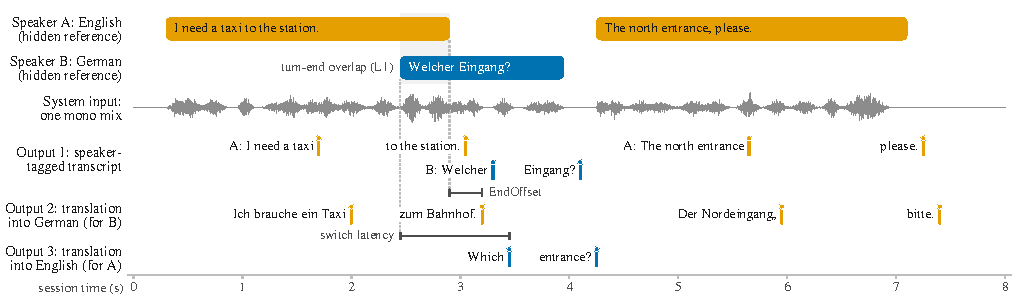
\includegraphics[width=\textwidth]{figures/fig1_task.pdf}
  \caption{\task on one mono stream (illustrative; invented utterances). Speakers A (English) and B (German) share one device. The system hears only the mix and must emit, without retraction, translations into each listener's language, choosing the direction itself, and may also emit a speaker-tagged transcript (Output 1). Ticks mark committed pieces at their emission time, coloured by the speaker whose speech they render. \eo (\emph{end offset}): time from the end of a turn to the last word of its translation, i.e., how long the listener waits. \emph{Switch latency}: time from the start of a turn in the new direction to the first word of its translation. Grey band: turn-end overlap (condition L1). Reference turns are hidden from the system and used only for scoring (\cref{sec:bench} defines the metrics).}
  \label{fig:task}
\end{figure*}

Two people who share no language can talk through a device that translates both sides, a goal of early speech translation systems \citep{waibel1996interactive,lavie1996translation,wahlster2000verbmobil} that deployed services such as Skype Translator have since offered \citep{lewis2015skype}.
The device stands in for a dialogue interpreter, who coordinates turns as well as translating them \citep{wadensjo1998interpreting,roy2000interpreting}.
Conversation leaves it little time: gaps between turns are of the order of 200\,ms while producing language takes over 600\,ms \citep{levinson2015timing}, average gaps lie within 250\,ms of the cross-language mean in 10 languages \citep{stivers2009universals}, and about 40\% of between-speaker intervals are overlaps \citep{heldner2010pauses}.
Simultaneous speech translation (SimulST) has matured from wait-$k$ and monotonic attention \citep{ma2019stacl,ma2020monotonic,ma2020simulmt} through local-agreement and attention-based policies, also for unbounded audio \citep{liu2020lowlatency,polak2022cuni,papi2023alignatt,papi2024streamatt}, to large streaming models \citep{seamless2023seamless,ouyang2025infinisst,labiausse2025highfidelity}, and IWSLT now evaluates it on long unsegmented audio \citep{abdulmumin2025findings,adelani2026speech}.
Yet most work uses human pre-segmented speech \citep{papi2025how}, and SimulST benchmarks, segmented or not, translate one source language in one fixed direction, mostly from a single speaker.

Conversation changes the problem in four ways (\cref{fig:task}).
(i)~\emph{The direction is latent}: one device hears both speakers in one mono stream, so the system must find, as it listens, each change of speaker and hence which way to translate. With one language per speaker, as in our scope, this is spoken language identification, but changes must be detected within gaps of a few hundred milliseconds or during overlap.
(ii)~\emph{Turns are short and close}: the median turn in our real dialogues lasts 2.86\,s after silence trimming, and in natural conversation a reply follows after a short gap or overlaps the end of the turn it answers.
(iii)~\emph{Output is committed}: a listener may reply as soon as text appears, and a later revision cannot undo that reply, so we score append-only output; re-translation systems \citep{arivazhagan2020retranslation} take part through a commit rule such as local agreement (\cref{sec:exp-setup}).
(iv)~\emph{Latency is felt at turn ends}: the listener waits after each turn (\eo) and at each change of direction (switch latency), beyond the lag within a turn that \laal measures \citep{papi2024streamatt}.
We therefore pose \taskfull (\task) as streaming structured prediction from a mixture, with a latent speaker and direction state and append-only, time-stamped emissions on several channels: a translation into each language and, optionally, a speaker-attributed transcript and speaker activity.

Prior systems cover parts of this setting (\cref{tab:positioning}).
JSTAR \citep{moritz2025transcribing} jointly streams recognition and translation of bilingual conversations and also infers who speaks, wearer or partner, and hence the direction, but from spatial cues of multi-microphone smart glasses and on in-house data.
DiariST \citep{yang2024diarist} adds diarization to streaming translation of multi-speaker meetings, but only from Chinese to English.
STAC-ST \citep{zuluagagomez2023end} handles two speakers in one channel with speaker-turn tokens, but offline and from one source language.
Seed LiveInterpret~2.0 \citep{cheng2025seed} names multi-speaker confusion as a challenge and depicts a bilingual conversation, but this closed system is evaluated per direction without overlap and covers only Chinese--English, which \bench lacks, so we do not run it.
We claim neither single-channel input nor conversational translation as new.
To our knowledge, however, no public benchmark evaluates streaming translation of both sides of a two-language conversation from one mono stream, where speaker changes, directions and turn ends are latent and turns may overlap, and no open baselines or models exist for this setting.

We ask (\textbf{RQ1}) how much of the difficulty lies in segmentation and routing (choosing each turn's direction) rather than translation; (\textbf{RQ2}) how quality, lag within a turn and listener wait trade off as turn-taking tightens from mediated to natural gaps and turn-end overlap, and for a distant language pair; (\textbf{RQ3}) whether one streaming model that writes transcripts and translations into one token stream closes the gap between oracle and realistic segmentation without oracle input; and (\textbf{RQ4}) whether synthetic sessions rank systems as real ones do.
Our contributions are:
\begin{itemize}
  \item \textbf{Task and protocol} (\cref{sec:task}): \task with irrevocable, time-stamped outputs whose language encodes the direction, scored under oracle and realistic segmentation.
  \item \textbf{\bench} (\cref{sec:bench}): 86 German--English telephone dialogues (\taxi) with real speech, 640 human-translated turns and rendered timing \citep{bas2001taxi}, shipped as deterministic build scripts and checksums, and an evaluation-only synthetic \pair{En}{De} and \pair{Ko}{En} track (\syn); both are rendered with natural gaps (L0) and with turn-end overlap (L1), the real track also with translation-mediated gaps (L0). \draftnote{planned; \syn and the L1 renders are not built yet}
  \item \textbf{A scorer and its validation protocol} (\scorer; \cref{sec:bench}) for per-direction quality, \laal, \eo, switch latency and wrong-direction output, plus cpWER and DER, tested by controlled perturbations. \draftnote{partly planned; v0.1 computes BLEU, chrF, \laal, \eo, empty turns and wrong-language words given turn IDs; only two perturbation rows exist, as preliminary runs, and the untranslated-source row exposes a \laal{} artefact (\cref{tab:sanity})}
  \item \textbf{A controlled study} (\cref{sec:exp}) of strong open systems under oracle and realistic wrappers, with an oracle-component factorial over segmentation, routing and overlap. \draftnote{planned; only offline oracle cascades have been run}
  \item \textbf{\model} (\cref{sec:model}): an open streaming speech LLM that writes speaker-tagged transcripts and direction-tagged translations into one token stream on an 80\,ms clock and commits translations at alignment-verified meaning units; ablations test whether coupling turn-taking and translation decisions helps. \draftnote{planned; only the streaming ASR backbone is built}
\end{itemize}
Given oracle turns, an offline ASR$\rightarrow$LLM cascade reaches \prelim{42.66} (\ende) and \prelim{28.11} (\deen) BLEU on \taxi ($^\dagger$preliminary; to be re-run under the final protocol).
Without oracle turns, the best open pipeline loses \tbdtext{} COMET, segmentation and routing explain \tbdtext{}\% and \tbdtext{}\% of this loss, \model recovers \tbdtext{}\% of it, and Kendall's $\tau$ between synthetic and real system rankings is \tbdtext{}.

\textbf{Scope.} We study two speakers, two languages and text output, under natural gaps, mediated gaps and turn-end overlap; interruptions and barge-in, more than two speakers, code-switching and speech output are left to future work.
